\documentclass{beamer}
\usepackage[utf8]{inputenc}
\usepackage{graphicx}

\newtheorem{definicion}{Definición}
\newtheorem{ejemplo}{Ejemplo}

%%%%%%%%%%%%%%%%%%%%%%%%%%%%%%%%%%%%%%%%%%%%%%%%%%%%%%%%%%%%%%%%%%%%%%%%%%%%%%%
\title[Método de la bisección]{Método de la bisección aplicado a la función $f(x)=5^x-5$}
\author[Claudia, Cathaysa, Carlos]{Claudia Ballester Niebla, Cathaysa Pérez Quintero y Carlos Herrera Carballo}
\date[14-05-2014]{14 de mayo de 2014}
%%%%%%%%%%%%%%%%%%%%%%%%%%%%%%%%%%%%%%%%%%%%%%%%%%%%%%%%%%%%%%%%%%%%%%%%%%%%%%%

\usetheme{Madrid}
%\usetheme{Antibes}
%\usetheme{tree}
%\usetheme{classic}

\definecolor{pantone254}{RGB}{122,59,122}
\definecolor{pantone3015}{RGB}{0,88,147}
\definecolor{pantone432}{RGB}{56,61,66}
\setbeamercolor*{palette primary}{use=structure, fg=white,bg=pantone254}
\setbeamercolor*{palette secondary}{use=structure, fg=white,bg=pantone3015}
\setbeamercolor*{palette tertiary}{use=structure, fg=white,bg=pantone432}
%%%%%%%%%%%%%%%%%%%%%%%%%%%%%%%%%%%%%%%%%%%%%%%%%%%%%%%%%%%%%%%%%%%%%%%%%%%%%%%
\begin{document}
  
%++++++++++++++++++++++++++++++++++++++++++++++++++++++++++++++++++++++++++++++
\begin{frame}

  
  \titlepage

  \begin{small}
    \begin{center}
     Facultad de Matemáticas \\
     Universidad de La Laguna
    \end{center}
  \end{small}

\end{frame}
%++++++++++++++++++++++++++++++++++++++++++++++++++++++++++++++++++++++++++++++

%++++++++++++++++++++++++++++++++++++++++++++++++++++++++++++++++++++++++++++++
\begin{frame}
  \frametitle{Índice}
  \tableofcontents[pausesections]
\end{frame}
%++++++++++++++++++++++++++++++++++++++++++++++++++++++++++++++++++++++++++++++
\section{Objetivos}
\begin{frame}
\frametitle{Objetivos}
\begin{itemize}
  \item {\bf Objetivo principal}: Implementación con Python del método de bisección.\pause
  \item {\bf Objetivo específico}: Cómo se aproximan las raíces de una función, mediante el método de bisección.
\end{itemize}
\end{frame}
%++++++++++++++++++++++++++++++++++++++++++++++++++++++++++++++++++++++++++++++

\section{Fundamentos teóricos}
\begin{frame}
\frametitle{Fundamentos teóricos. Método de bisección.}
El método de la bisección se basa en dos teoremas, el de Bolzano y el del Valor Intermedio.\pause
\begin{definicion}
\begin{itemize}
\item Teorema de Bolzano: Sea $f(x)$ una función continua en un intervalo [a,b] tal que $f(a)*f(b)<0$, entonces existe un punto c perteneciente al intervalo (a,b) tal que $f(c)=0$.\pause
\item Teorema del Valor Intermedio: Sea $f(x)$ una función continua en un intervalo [a,b], tal que $f(a)<f(b)$ entonces, para todo k tal que $f(a)<k<f(b)$ existe $x_0$ que pertenece al intervalo (a,b) tal que $f(x_0)=k$.
\end{itemize}
\end{definicion}

\end{frame}

\begin{frame}
\frametitle{Fundamentos teóricos. Método de bisección.}
\begin{definicion}
Dados dos puntos a y b, tal que $f(a)$ y $f(b)$ tengan signos distintos debe tener, al menos, una raíz en el intervalo [a,b]. Este método divide el intervalo en dos utilizando un tercer punto c= $\frac{a+b}{2}$. De esta forma, se darán dos posibilidades: $f(a)$ y $f(c)$, ó $f(c)$ y $f(b)$ tienen distinto signo. Se aplica este método al subintervalo donde ocurre el cambio de signo. Así se realizará tantas veces como sea necesario para conseguir la máxima precisión.
\end{definicion}
\end{frame}
%++++++++++++++++++++++++++++++++++++++++++++++++++++++++++++++++++++++++++++++

\section{Procedimiento experimental}
\begin{frame}
\frametitle{Procedimiento experimental.}
{\LARGE Descripción de los experimentos.}
\begin{itemize}
\item {\bf Experimento 1:} Con el fin de verificar la precisión del algoritmo propuesto, se ejecuta el programa con los mismos valores y la misma función tres veces. De esta forma, si los resultados coinciden, significará que es exacto.\pause
\item {\bf Experimento 2:} Se ejecutará el algoritmo con distintas funciones para así observar que es válido para cualquier $f(x)$.\pause
\item {\bf Experimento 3:} En este tercer experimento, se ejecutará el programa con distintos intervalos para verificar la existencia de raíces en los mismos.\pause
\item {\bf Experimento 4:} Se observa cómo varían las soluciones obtenidas con distintos valores de tolerancia de error.\pause
\item {\bf Experimento 5:} Para determinar el rendimiento del algoritmo, se introduce un cronómetro en el mismo, de forma que imprima el tiempo que tarda la CPU de la computadora en ejecutar el programa.
\end{itemize}
\end{frame}
%++++++++++++++++++++++++++++++++++++++++++++++++++++++++++++++++++++++++++++++

\begin{frame}

\frametitle{Procedimiento experimental.}
{\LARGE Resultados.}

\textbf{Experimento 1}
\begin{table}[!ht]
\begin{center}
\begin{tabular}{|c|c|}\hline
{\bf Intento} & {\bf Resultado}\\ \hline
1 & 0.969\\
2 & 0.969\\
3 & 0.969\\
\hline
\end{tabular}
\end{center}
\caption{Tabla experimento 1}
\label{Mitabla}
\end{table}
\end{frame}

%++++++++++++++++++++++++++++++++++++++++++++++++++++++++++++++++++++++++++++++++
\begin{frame}
\frametitle{Procedimiento experimental.}
{\LARGE Resultados.}

\textbf{Experimento 2}
\begin{table}[!ht]
\begin{center}
\begin{tabular}{|c|c|}\hline
{\bf Funcion} & {\bf Resultado}\\ \hline
$5^x$ & Error\\
$5x-10$ & 1.969\\
$3x^2-1$ & Error\\
\hline
\end{tabular}
\end{center}
\caption{Tabla experimento 2}
\label{Mitabla2}
\end{table}
\end{frame}

%++++++++++++++++++++++++++++++++++++++++++++++++++++++++++++++++++++++++++++++++++++
\begin{frame}
\frametitle{Procedimiento experimental.}
{\LARGE Resultados.}

\textbf{Experimento 3}
\begin{table}[!h]
\begin{center}
\begin{tabular}{|c|c|}\hline
{\bf Intervalo} & {\bf Resultado}\\ \hline
(-3,2) & 1.023\\
(-2,3) & 1.008\\
(2,5) & Error\\%No hay raíces en el intervalo
\hline
\end{tabular}
\end{center}
\caption{Tabla experimento 3}
\label{Mitabla3}
\end{table}
\end{frame}

%+++++++++++++++++++++++++++++++++++++++++++++++++++++++++++++++++++++++++++++++++++++
\begin{frame}
\frametitle{Procedimiento experimental.}
{\LARGE Resultados.}

\textbf{Experimento 4}
\begin{table}[!ht]
\begin{center}
\begin{tabular}{|c|c|}\hline
{\bf Tolerancia} & {\bf Resultado}\\ \hline
0.01 & 0.996\\
0.02 & 0.992\\
0.001 & 1.000\\
\hline
\end{tabular}
\end{center}
\caption{Tabla experimento 4}
\label{Mitabla4}
\end{table}
\end{frame}
%++++++++++++++++++++++++++++++++++++++++++++++++++++++++++++++++++++++++++++++
\begin{frame}
\frametitle{Procedimiento experimental.}
{\LARGE Resultados.}

\textbf{Experimento 5}
\begin{table}[!ht]
\begin{center}
\begin{tabular}{|c|c|} \hline
\textbf{Intento} & \textbf{Tiempo (segundos)} \\ \hline
1 & $2.8133*10^-5$ \\%Pidiendo el programa
2 & $2.4080*10^-5$ \\%Puestos directamente usuario
3 & $3.1948*10^-5$ \\%Puestos por consola e intervalo -10,10
\hline
\end{tabular}
\end{center}
\caption{Tabla experimento 5}
\label{Mitabla5}
\end{table}
\end{frame}
%+++++++++++++++++++++++++++++++++++++++++++++++++++++++++++++++++++++++++++++++++++++++++
\section{Algoritmo}
\tiny{
\begin{verbatim}
Algoritmo empleado
import time
import timeit
def f(x):
  return (5**x)-5
def biseccion(a,b,tol):
  c=(a+b)/2.0
  while((f(c)!=0.000001) and (abs(b-a)>tol)):
    if f(a)*f(c)<0.000001:
      b=c
    else:
      a=c
    c=(a+b)/2.0
  return c

import sys
if (len(sys.argv)==4):
  A=float(sys.argv[1])
  B=float(sys.argv[2])
  TOL=float(sys.argv[3])
else:
  A=float(raw_input("Introduzca el extremo a del intervalo: "))
  B=float(raw_input("Introduzca el extremo b del intervalo: "))
  TOL=float(raw_input("Introduzca la tolerancia del error que desee: "))
if f(A)*f(B)<0.000001:
  start=time.time()
  raiz=biseccion(A,B,TOL)
  finish=time.time()-start
  print "El tiempo de ejecución es:"
  print finish
  print "La raíz aproximada de la función escogida es: %4.3f" %raiz
else:
  print "En ese intervalo no existe raíz, por favor vuelva a ejecutar el programa con otros valores"
\end{verbatim}
}
\section{Gráficas}
\begin{frame}
\begin{figure}[!th]
\begin{center}
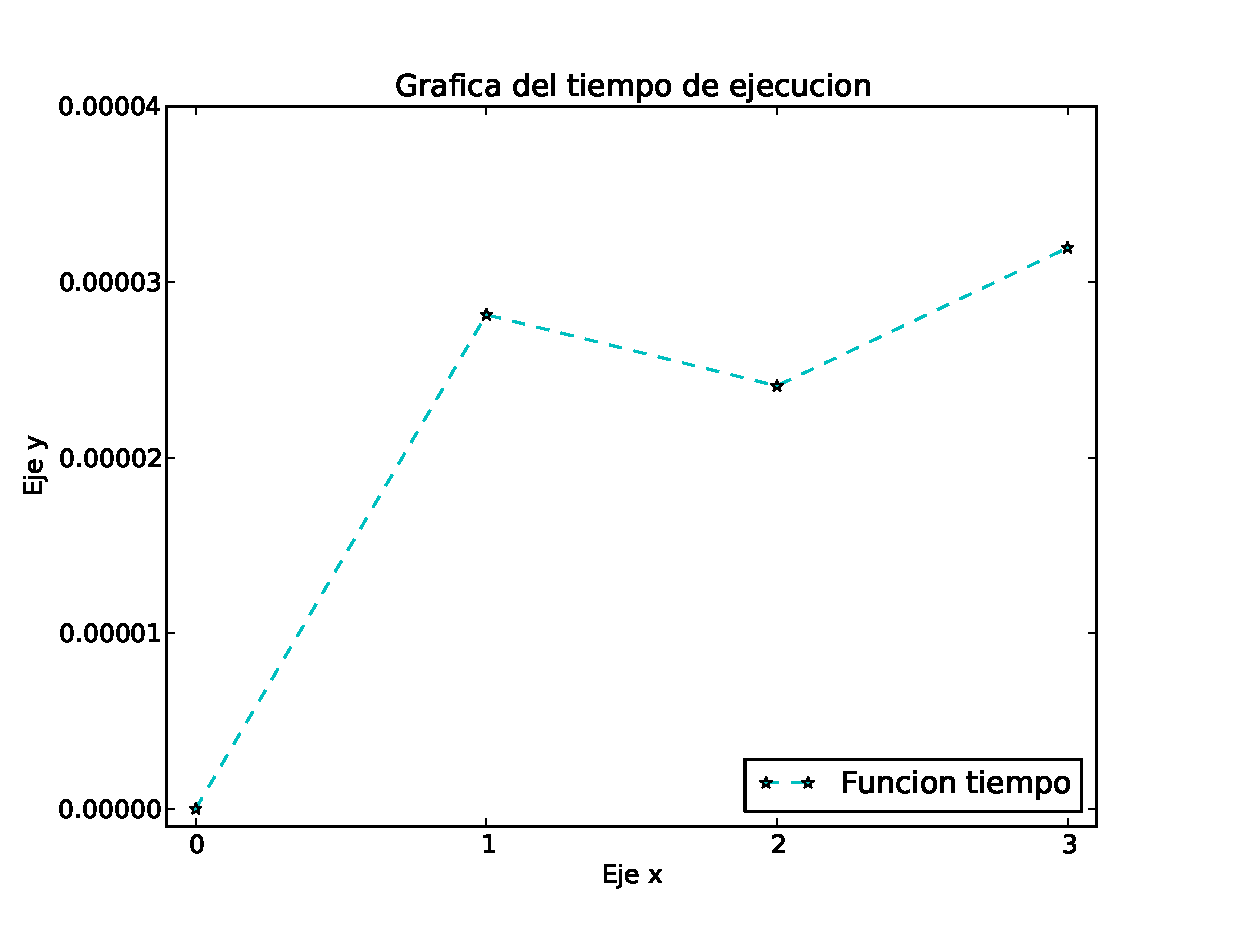
\includegraphics[width=0.75\textwidth]{graftime.eps}
\caption{Gráfica del tiempo}
\label{fig:1}
\end{center}
\end{figure}
\end{frame}

\begin{frame}
\begin{figure}[!th]
\begin{center}
\includegraphics[width=0.75\textwidth]{grafcap2.eps}
\caption{Gráfica de la funcion}
\label{fig:1}
\end{center}
\end{figure}
\end{frame}
%++++++++++++++++++++++++++++++++++++++++++++++++++++++++++++++++++++++++++++++
\section{Conclusiones}
\begin{frame}
\begin{center}
\begin{enumerate}
\item {\LARGE Eficacia para la función propuesta.}\pause

\item {\LARGE Conflicto en casos de funciones con más de una raíz.}\pause

\item {\LARGE Casos de dos raíces o más:}\pause

\begin{itemize}
\item Escoger distintos intervalos.\pause
\item Raíz única dentro de cada uno de los intervalos.
\end{itemize}
\end{enumerate}
\end{center}
\end{frame}
%++++++++++++++++++++++++++++++++++++++++++++++++++++++++++++++++++++++++++++++++
\section{Bibliografía}
%++++++++++++++++++++++++++++++++++++++++++++++++++++++++++++++++++++++++++++++
\begin{frame}
  \frametitle{Bibliografía}

  \begin{thebibliography}{10}
\bibitem[Gu\'ia Docente, 2013]{guia}
    Gu\'ia docente de la asignatura: T\'ecnicas Experimentales.
    (2013)
    
    {\tiny $http://eguia.ull.es/matematicas/query.php?codigo=299341201$}
\bibitem[C\'alculo Infinitesimal]{spivak}
    Spivak,~M.~-Calculus,~ Ed. Cambridge,~ 2006;~ Ed.~Revert\'e,~ 1981~ [BULL]
\bibitem[M\'etodo de Bisecci\'on]{web}
  Demostraci\'on del M\'etodo de Bisecci\'on.
  (2008)
  
  {\tiny $http://www.ma3.upc.edu/users/carmona/teaching/clases/08-09/trabajos/$}
\bibitem[Tutorial de Python]{python}
  Python para todos. ~-Ra\'ul Gonz\'alez Duque.
  
  {\tiny $http://campusvirtual.ull.es/1314/pluginfile.php/197675/mod_resource/content/4/Primera_Parte/General2012/Python_para_todos.pdf$}
\bibitem[Tutorial de \LaTeX{}]{latex}
  The beamer class. ~User Guide for version 3.26.
  
  {\tiny $http://campusvirtual.ull.es/1314/pluginfile.php/197674/mod_resource/content/1/beameruserguide.pdf$}
  \end{thebibliography}
\end{frame}
\end{document}

%++++++++++++++++++++++++++++++++++++++++++++++++++++++++++++++++++++++++++++++